\section{РЕЗУЛЬТАТЫ ВИЗУАЛИЗАЦИИ}
\label{sec:visualization}


Для большей наглядности были решено визуализировать только те жанры, которые лучше всего выделяются всеми алгоритмами классификации. Из 10 жанров были выбраны следующие:
\begin{itemize}
\item классическая музыка;
\item музыка в жанре металл;
\item музыка в жанре поп.
\begin{itemize}

Визуализация проводилась над фрагментами музыкального произведения

\subsection{Метод главных компонент} % (fold)
\label{sub:pca}
Метод главных компонент -- один из основных способов уменьшить размерность данных, потеряв наименьшее количество информации. Применяется во многих областях, таких как распознавание образов, компьютерное зрение, сжатие данных и т. п. Вычисление главных компонент сводится к вычислению собственных векторов и собственных значений ковариационной матрицы исходных данных или к сингулярному разложению матрицы данных. 



По двумерному отображению данных видно, что кластеры ярко выражены и линейно разделимы. Особой компактностью отличается музыка в жанре поп. Кластеры с классической музыкой и с музыкой в жанре металл, также ярко выражены.
\begin{figure}[h]
\centering
  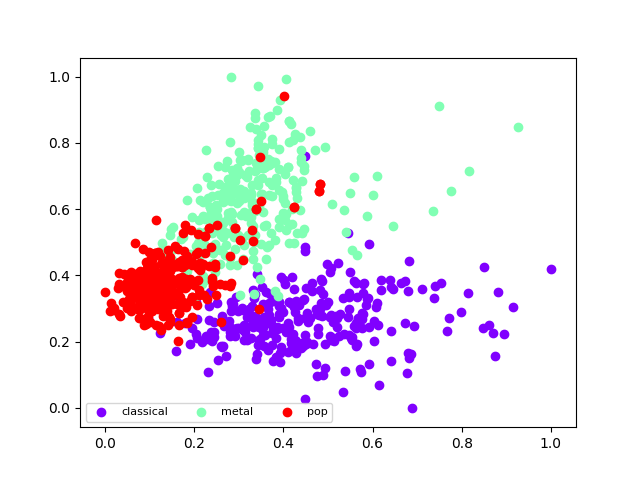
\includegraphics{2dpca.png}
  \caption{Отображения пространства  признаков музыкальных треков в двухмерное простарнство алгоритмом PCA.}
  \label{fig:results:2dtsne}
\end{figure}

Трёхмерное отображение показывает те же результаты, что и двумерная. В обоих проекциях виден малый зазор между классами.

\begin{figure}[h]
\centering
  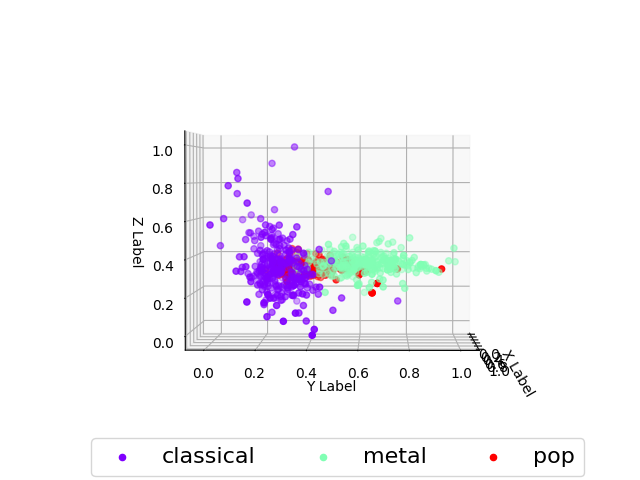
\includegraphics{3dpca1.png}
  \caption{Отображения пространства  признаков музыкальных треков в трёхмерное пространство алгоритмом PCA. Первая проекция. }
  \label{fig:results:2dtsne}
\end{figure}


\begin{figure}[h]
\centering
  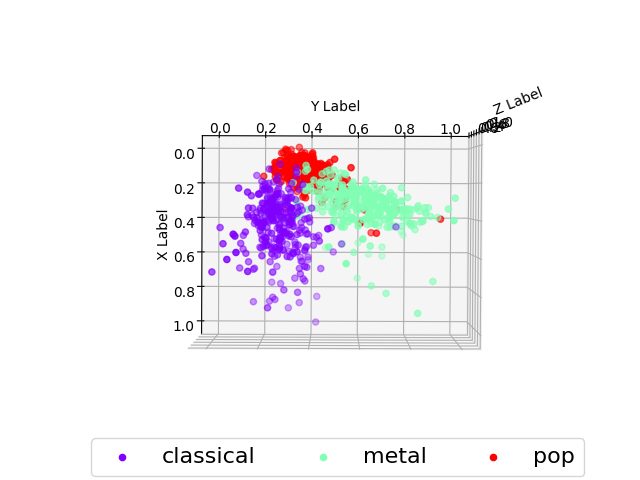
\includegraphics{3dpca2.png}
  \caption{Отображения пространства  признаков музыкальных треков в трёхмерное пространство алгоритмом PCA. Вторая проекция. }
  \label{fig:results:2dtsne}
\end{figure}


% subsection pca (end)
\subsection{t-SNE} % (fold)
\label{sub:tsne}

\end{itemize}
\begin{figure}[h]
\centering
  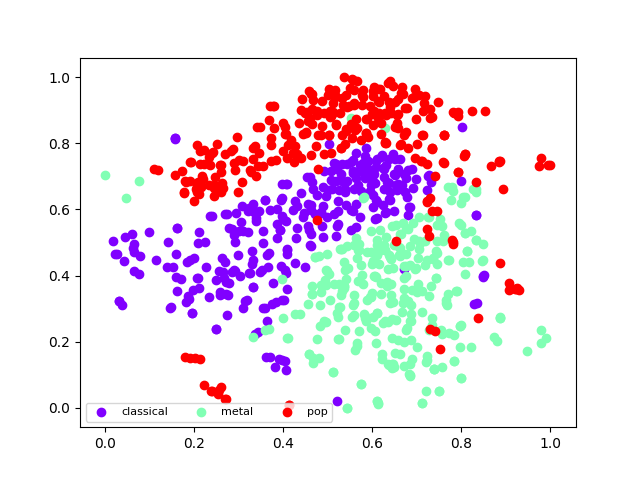
\includegraphics{vis1.png}
  \caption{Отображения пространства  признаков музыкальных треков в двухмерное простарнство алгоритмом t-SNE.}
  \label{fig:results:2dtsne}
\end{figure}

\begin{figure}[h]
\centering
  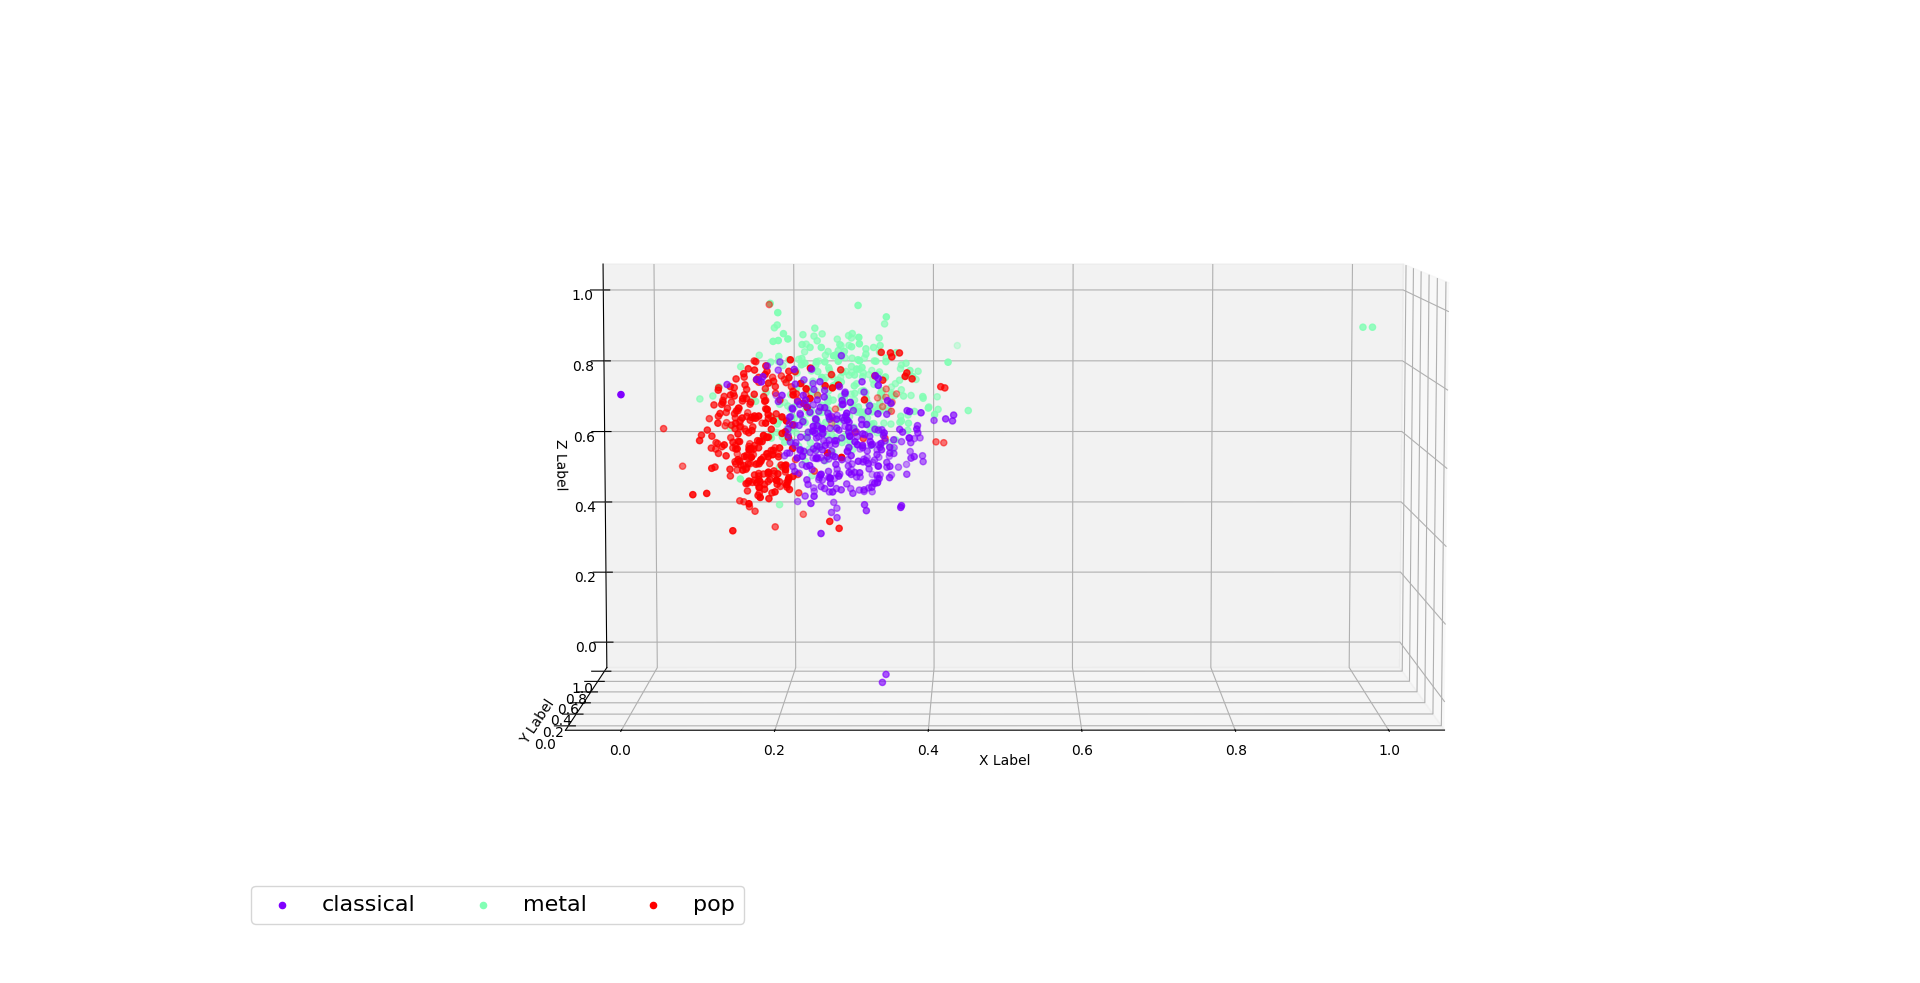
\includegraphics[scale=0.5]{3dtsne1.png}
  \caption{Отображения пространства  признаков музыкальных треков в трёхмерное пространство алгоритмом t-SNE. Первая проекция. }
  \label{fig:results:2dtsne}
\end{figure}


\begin{figure}[h]
\centering
  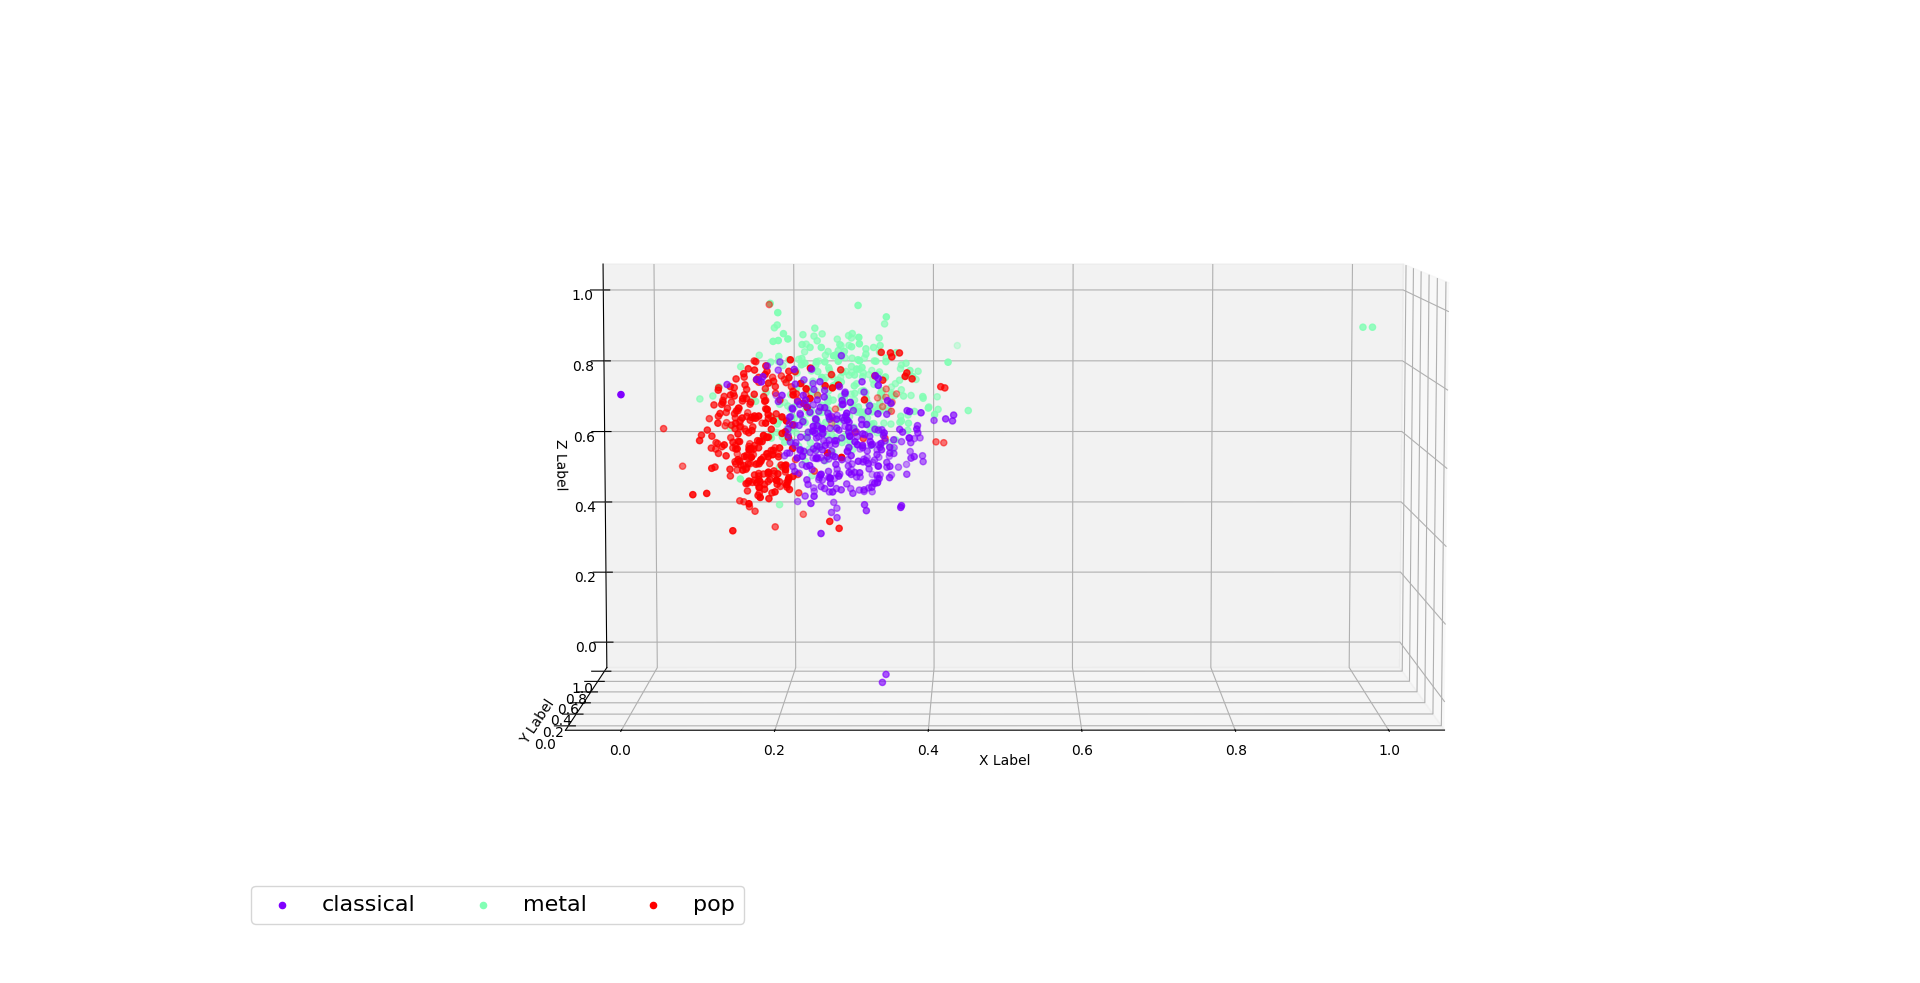
\includegraphics[scale=0.5]{3dtsne1.png}
  \caption{Отображения пространства  признаков музыкальных треков в трёхмерное пространство алгоритмом t-SNE. Вторая проекция. }
  \label{fig:results:2dtsne}
\end{figure}

Визуализация также показала, что выделенные информационные образы значимы и на их основе можно делать рекомендательный сервис. 